\documentclass[conference]{IEEEtran}
\usepackage[utf8]{inputenc}
\usepackage[T1]{fontenc}
\usepackage{graphicx}
\usepackage{booktabs}
\usepackage{siunitx}
\usepackage{url}
\usepackage{tikz}
\usetikzlibrary{arrows.meta,positioning,fit,backgrounds}
\usepackage{hyperref}
\hypersetup{colorlinks=true,linkcolor=black,citecolor=black,urlcolor=blue}
\graphicspath{{figures/}}

\title{A Word-Level Vibrotactile Vest for Delivering Spoken Sinhala to Deaf Users:\\Design, Encoding and Evaluation Protocol}

\author{\IEEEauthorblockN{Dilan Perera}
\IEEEauthorblockA{Intelligent Systems \& Mechatronics Research Laboratory (ISMR Labs)\\
Colombo, Sri Lanka\\
\url{https://github.com/ISMR-Labs/Sinhala-Speech-to-Haptic-System-for-the-Hearing-Impaired}}}

\begin{document}
\maketitle

\begin{abstract}
About 390\,000 Sri Lankans have a hearing difficulty, most of them in Sinhala-speaking households where no standardised sign language is shared with hearing family members. We describe a wearable system that lets a deaf person feel spoken Sinhala as vibration. A laptop recognises speech with a Sinhala-tuned Whisper model and maps each recognised word of a closed vocabulary to a short vibrotactile pattern, which an ESP32-S3 controller plays on 18 coin-motor modules arranged as two $3\times3$ grids on the chest and upper back of a vest. Rather than coding phonemes, as recent tactile speech displays do, the system codes whole words as two \SI{200}{ms} frames of one or two active motors, which keeps every pattern inside the \SIrange{3}{4}{cm} spatial acuity of the torso and gives a codebook whose minimum pairwise distance is two of three cues for a 20-word vocabulary. We present the hardware, the encoding and its justification from the vibrotactile literature, the host pipeline, and the protocol of a learnability study with hearing and deaf participants. The 17-module prototype, firmware, host software, codebook and study tools are released as an open repository. No perception results are reported yet; the paper documents the design and the evaluation plan.
\end{abstract}

\begin{IEEEkeywords}
vibrotactile display, sensory substitution, haptic communication, deaf, Sinhala, speech recognition, wearable, ESP32
\end{IEEEkeywords}

\section{Introduction}
The 2012 census of Sri Lanka counted 389\,077 persons with hearing difficulty, 21 per 1000 of the population \cite{census2012}. Advocacy groups put the number of deaf and hard-of-hearing people at about 400\,000 and the number of recognised sign-language interpreters in the low tens; the Sinhala-speaking deaf community does not share a fully standardised sign language with the hearing people around it. In a typical household the hearing members speak Sinhala and the deaf member lip-reads, writes, or is left out.

Delivering speech through the skin has a long history. Geldard's Vibratese used five chest vibrators with three durations and three intensities, and trained readers exceeded 35 words per minute \cite{geldard1957}. Tactile aids of the 1980s and 1990s transmitted spectral features of speech as a supplement to lip-reading, with mixed adoption \cite{summers1992}. The most complete recent system, TAPS, codes the 39 English phonemes as spatial and movement patterns on 24 forearm tactors; ten adults reached 86\,\% phoneme recognition after one to four hours of training \cite{reed2019}, and the best learners acquired 500 words at about one word per minute \cite{tan2020}. Sound-to-touch devices for the deaf take a different route, mapping frequency bands of ambient sound to motors on the torso or wrist \cite{novich2015,perrotta2021}; they convey that a sound happened and its character, not its words.

None of these systems exists for Sinhala, and none fits the situation of a deaf family member who needs a small set of words reliably. Our design question is therefore narrow: can a low-cost vest with 18 vibration modules deliver a closed vocabulary of spoken Sinhala words that a wearer can learn in a few sessions and identify reliably? This paper gives the design and the plan to answer it.

\section{Related Work and Design Constraints}
Three results from the vibrotactile literature bound the design.

\textbf{Spatial acuity on the torso.} Van Erp measured \SIrange{3}{4}{cm} acuity for successive stimuli over most of the torso, with stimulus onset asynchrony as the main timing factor, and absolute localisation within about \SI{5}{cm} \cite{vanerp2005acuity,vanerp2005directions}. J{\'o}hannesson et al. found relative acuity down to \SI{13}{mm} spacing in a two-alternative task \cite{johannesson2017}. Localisation is best near anatomical landmarks such as the midline \cite{cholewiak2004}. A $3\times3$ grid at \SI{80}{mm} pitch, centred on the midline, is therefore conservative.

\textbf{Pattern recognition on the torso.} Jones, Lockyer and Piateski report 99--100\,\% identification for seven of eight simple patterns on a torso array, better than on the forearm and unaffected by walking \cite{jones2006}. Simple spatial patterns on the torso are nearly error-free; complexity, not the site, is the limit.

\textbf{Throughput.} Novich and Eagleman estimated the achievable information rate of the skin with spatiotemporal codes on the back and concluded that it falls below the \SIrange{64}{110}{bit/s} that continuous speech requires \cite{novich2015}. Phoneme-level coding reaches practical word rates of about one per minute even after extended training \cite{tan2020}.

Together these argue for word-level codes on a coarse torso grid: patterns the skin resolves without error, a vocabulary chosen for need rather than coverage, and no attempt at phoneme streams. Coin eccentric-rotating-mass (ERM) motors vibrate at \SIrange{150}{200}{Hz}, on the sensitive part of the Pacinian channel that peaks near \SI{250}{Hz} \cite{makous1995}, and are cheap and robust; their \SIrange{50}{100}{ms} spin-up sets a lower bound on frame length.

\section{System Design}

\subsection{Architecture}
\begin{figure}[t]
\centering
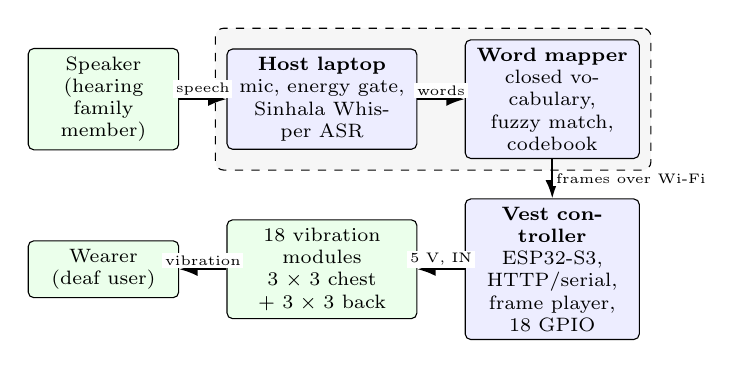
\begin{tikzpicture}[font=\scriptsize, >=Latex, node distance=4mm,
  box/.style={draw, rounded corners=2pt, align=center, inner sep=3pt, minimum height=14pt, fill=white},
  ext/.style={box, fill=green!8}, comp/.style={box, fill=blue!7}, lbl/.style={font=\tiny, fill=white, inner sep=1pt, align=center}]
\node[ext, text width=1.7cm] (spk) {Speaker\\(hearing family member)};
\node[comp, right=6mm of spk, text width=2.2cm] (asr) {\textbf{Host laptop}\\mic, energy gate,\\Sinhala Whisper ASR};
\node[comp, right=6mm of asr, text width=2.0cm] (map) {\textbf{Word mapper}\\closed vocabulary,\\fuzzy match, codebook};
\node[comp, below=5mm of map, text width=2.0cm] (ctl) {\textbf{Vest controller}\\ESP32-S3, HTTP/serial,\\frame player, 18 GPIO};
\node[ext, left=6mm of ctl, text width=2.2cm] (motors) {18 vibration modules\\$3\times3$ chest + $3\times3$ back};
\node[ext, left=6mm of motors, text width=1.7cm] (user) {Wearer\\(deaf user)};
\begin{scope}[on background layer]
\node[draw, dashed, rounded corners=3pt, fill=gray!7, fit=(asr)(map), inner sep=4pt] (host) {};
\end{scope}
\draw[->, thick] (spk) -- node[lbl, above]{speech} (asr);
\draw[->, thick] (asr) -- node[lbl, above]{words} (map);
\draw[->, thick] (map) -- node[lbl, right]{frames over Wi-Fi} (ctl);
\draw[->, thick] (ctl) -- node[lbl, above]{5 V, IN} (motors);
\draw[->, thick] (motors) -- node[lbl, above]{vibration} (user);
\end{tikzpicture}
\caption{System overview. Speech recognition and word mapping run on the laptop; the vest controller only plays timed frames.}
\label{fig:arch}
\end{figure}

Fig.~\ref{fig:arch} shows the pipeline. Recognition and vocabulary mapping run on a laptop so that the model can be swapped without reflashing; the vest controller is deliberately simple and plays frame sequences with its own timing, so network jitter does not disturb the rhythm inside a word.

\subsection{Vest hardware}
The vest carries 18 three-pin vibration modules (coin ERM motor with an on-board switching transistor) in 3D-printed pods, nine on the chest and nine on the upper back, each $3\times3$ at \SI{80}{mm} pitch (Fig.~\ref{fig:layout}). Pods are held on a two-layer sports vest with hook-and-loop patches so that the pitch can be adjusted per wearer. Each module's input is driven directly from a GPIO of an ESP32-S3 DevKitC; the 20 GPIOs used leave two spares. Modules share a \SI{5}{V} rail from a USB power bank; the normal load is two motors per frame (\SI{160}{mA}), the chase test is the only time all 18 run. The controller, power lead and a push button sit in a printed box at the hip. Module leads are \SI{1}{m} of three-core wire in \SI{4}{mm} braided sleeving. All enclosures are OpenSCAD parts in the repository.

\begin{figure}[t]
\centering
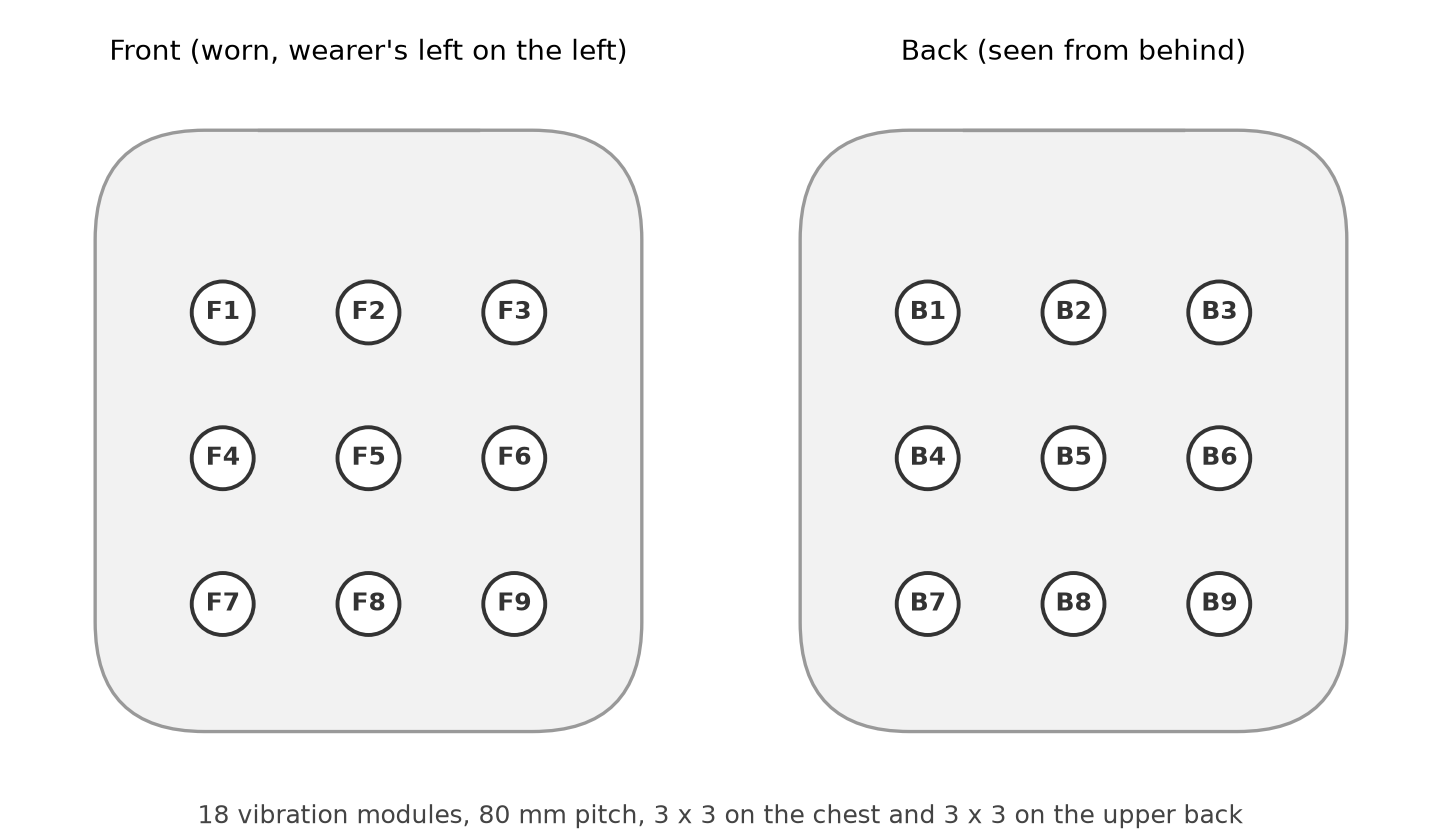
\includegraphics[width=\columnwidth]{motor-layout}
\caption{Motor layout. F1--F9 on the chest, B1--B9 on the upper back, \SI{80}{mm} pitch, centre column on the midline.}
\label{fig:layout}
\end{figure}

\subsection{Firmware}
The controller accepts one text protocol over HTTP (port 80, mDNS \texttt{vest.local}) and over USB serial: a sequence of frames \texttt{F <motors> <ms> <level>} separated by semicolons, a gap setting, stop, chase test and status. Frames are timed with the millisecond clock and up to 32 are buffered. Level is a \SI{100}{Hz} software PWM on the module input; with ERM motors it changes amplitude and frequency together, so the first vocabulary uses full level only. GPIO 3, 45 and 46 are strapping pins; the three-pin modules present a floating or weakly low input at reset, which was verified to boot normally.

\subsection{Encoding}
A word is two frames of \SI{200}{ms}, separated by \SI{80}{ms}, each frame switching on one motor or an adjacent horizontal or vertical pair on the same side of the body; words are separated by \SI{400}{ms}. The frame length exceeds the ERM spin-up, the gap lets the motor stop so the second frame is a separate event, and the alphabet of 18 singles plus 24 pairs gives $42^2 = 1764$ two-frame codes. Codes are assigned to words by a deterministic greedy search that maximises the minimum pairwise distance, defined as the sum over frame positions of the Jaccard distance between motor sets plus one when the front/back sequence differs; front-to-back movement is the easiest cue to feel. For the 20-word vocabulary in Table~\ref{tab:vocab} the minimum distance is 2.0 of a possible 3.0: every pair of words differs in at least two of its three cues. Fig.~\ref{fig:patterns} shows the first eight codes. Three reserved signals mark listening, an out-of-vocabulary word, and the end of an utterance.

\begin{table}[t]
\caption{Vocabulary v0: 20 words chosen for everyday exchanges in a household.}
\label{tab:vocab}
\centering
\small
\begin{tabular}{llll}
\toprule
Category & Words (romanised) & & \\
\midrule
Response & ow (yes) & naehae (no) & \\
Command & enna (come) & yanna (go) & nawathwanna (stop) \\
 & inna (wait) & & \\
Alert & udaw (help) & anathura (danger) & \\
Social & ayubowan (hello) & sthuthiyi (thanks) & hondayi (good) \\
Need & kanna (eat) & bonna (drink) & wathura (water) \\
Person & amma (mother) & thaththa (father) & \\
Question & koheda (where) & mokakda (what) & \\
Time & daen (now) & passe (later) & \\
\bottomrule
\end{tabular}
\end{table}

\begin{figure*}[t]
\centering
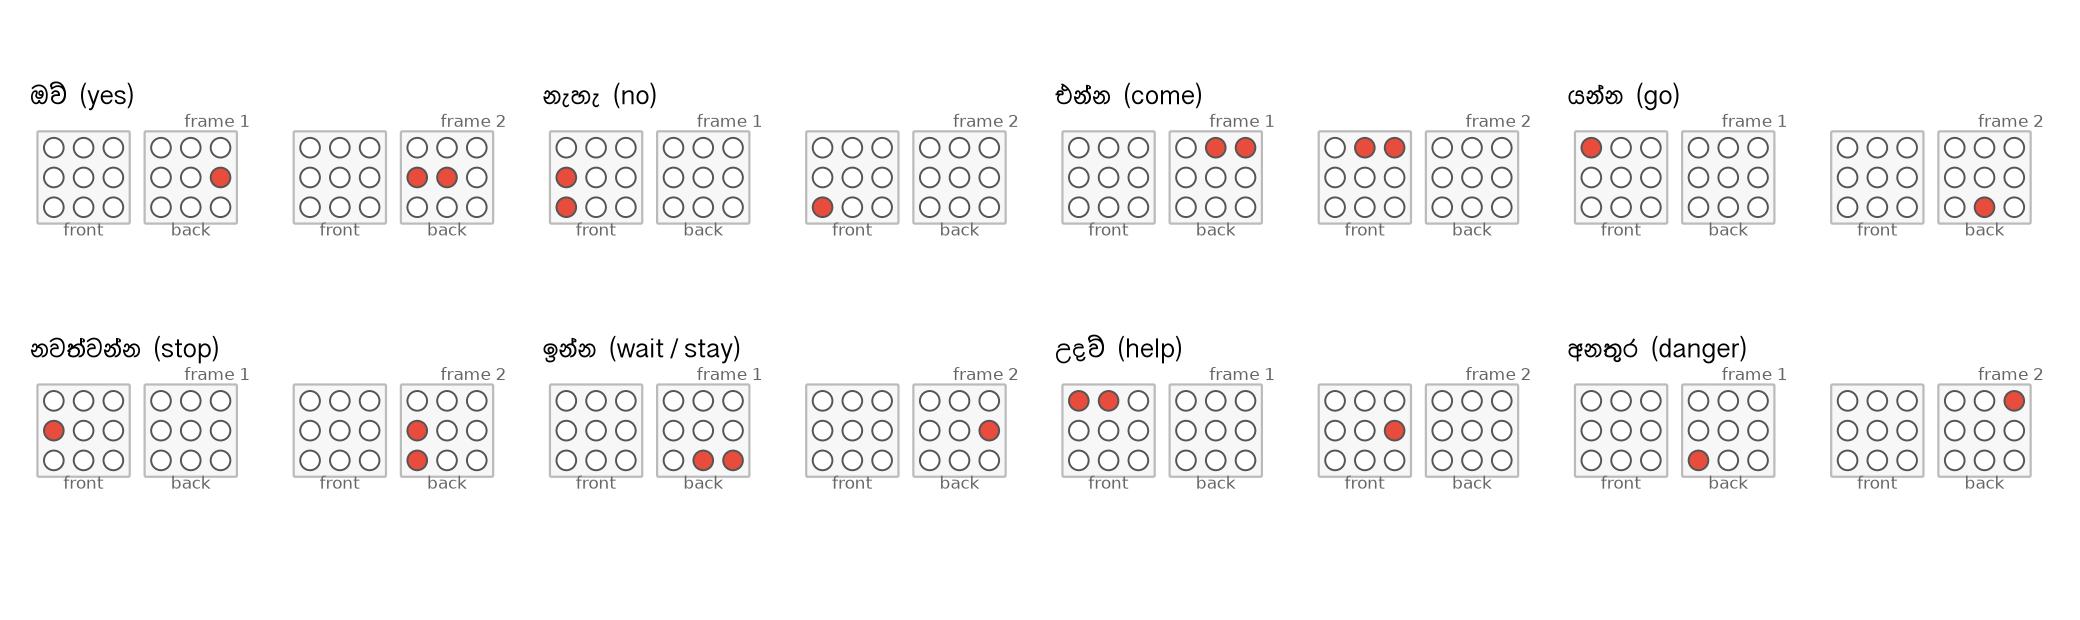
\includegraphics[width=0.92\textwidth]{patterns-example}
\caption{The first eight word codes. Each word is two frames of \SI{200}{ms}; filled circles are active motors on the front and back $3\times3$ grids.}
\label{fig:patterns}
\end{figure*}

\subsection{Speech pipeline}
The host captures the microphone at \SI{16}{kHz}, cuts utterances with an energy gate (\SI{0.7}{s} of silence ends an utterance), and transcribes with faster-whisper, the CTranslate2 port of Whisper \cite{radford2023}, with the language fixed to Sinhala. Whisper's multilingual base models are weak on Sinhala, so the pipeline accepts any fine-tuned checkpoint; public fine-tunes trained on the crowd-sourced Sinhala corpus (about 185\,000 utterances from 478 speakers \cite{kjartansson2018}, with the transcript refinements of \cite{warusawithana2022}) report word error rates of about \SIrange{22}{30}{\percent} on open text, and XLS-R fine-tunes \cite{babu2022} report \SIrange{24}{37}{\percent}. The vest does not need open-text accuracy: the recogniser output is matched against the 20-word vocabulary in Sinhala script, with a fuzzy match that tolerates a vowel-sign or final-letter error, and anything else is signalled as unknown. Closed-vocabulary accuracy will be measured on recordings of the 20 words from ten speakers before the user study, and a small keyword-spotting model is the fallback if it is insufficient.

\section{Evaluation Protocol}
The primary question is learnability. A pilot with eight hearing lab members, wearing ear defenders and masked by pink noise so that the motors cannot be heard, validates the codebook and procedure. The main study recruits 10 to 12 deaf or hard-of-hearing adults who read Sinhala, through the Sri Lanka Central Federation of the Deaf, with consent and instructions in Sinhala and Sri Lankan Sign Language. Each participant completes three sessions on separate days: familiarisation (each word twice with its label), two training blocks of 60 trials with feedback, a 60-trial identification test without feedback, and in the last session ten two- and three-word sentences for free recall. Sessions two and three begin with the test, giving 24 and \SI{48}{h} retention. Measures are identification accuracy, the learning curve, the $20\times20$ confusion matrix, reaction time and comfort. A word pair confused on more than 15\,\% of presentations is re-coded, accepted only if the minimum codebook distance does not fall. Success for this version is mean accuracy above 80\,\% at session three and no pair confused above 25\,\%. A second study will compare the distance-optimal codebook with a mnemonic one (for example \emph{come} as back-to-front motion), which may trade geometric separation for faster learning.

\section{Status}
Seventeen modules, their pods and the controller box have been built and wired on \SI{1}{m} leads; a chase test on the ESP32-S3 confirmed every module and the strapping-pin behaviour. The vest controller firmware compiles and implements the full protocol; the host tools play words and typed sentences on the hardware or on a terminal simulator, and run the microphone pipeline. The eighteenth module, the garment fitting, supply decoupling and the ASR closed-vocabulary test remain before the pilot. All design files, the codebook generator, the study protocol and the analysis script are in the repository.

\section{Discussion and Limitations}
The design trades vocabulary size for reliability. Twenty words cover calls, warnings, basic needs and two names; the two-frame alphabet has room for perhaps 40 words before perceptual separation falls, and three frames, a second intensity level, or a category-prefix frame can extend it. Whether deaf users prefer the arbitrary distance-optimal codes or mnemonic codes is an empirical question the second study addresses. ERM motors couple amplitude and frequency and start slowly; linear resonant actuators with a dedicated driver would allow faster, more uniform frames and a usable intensity dimension. The speech front end is the weakest link: Sinhala ASR is a low-resource problem, and the vest is only as good as the recogniser's accuracy on the vocabulary in a noisy home, which is why closed-vocabulary accuracy is measured first and keyword spotting is kept as a fallback. Finally, a torso display cannot replace sign language or captioning; its role is to let a deaf person receive a small set of important words from people who do not sign, in the moment, without looking.

\section{Conclusion}
We have presented a low-cost vest that delivers spoken Sinhala words as vibration patterns on the torso, grounded in what the vibrotactile literature says the skin can resolve, together with firmware, host software, a 20-word codebook with guaranteed separation, and a study protocol. The next step is the learnability study, whose results will be added to the repository.

\bibliographystyle{IEEEtran}
\bibliography{references}

\end{document}
